\subsection{System model}

\subsubsection{Coordinate}

To accurately locate the position of a slot, it is essential to establish a coordinate system. The coordinate system provides a framework for identifying the exact location of each slot within the warehouse space. By using a coordinate system, it is possible to implement a more efficient and organized storage system that can help streamline warehouse operations and optimize inventory management:
    \begin{equation}\label{eq:coordinate}
        X(i) = \text{ [Floor][Section][Location][Shelf][Column][Row]}
    \end{equation}

    \begin{figure}[!ht]
        \centering
        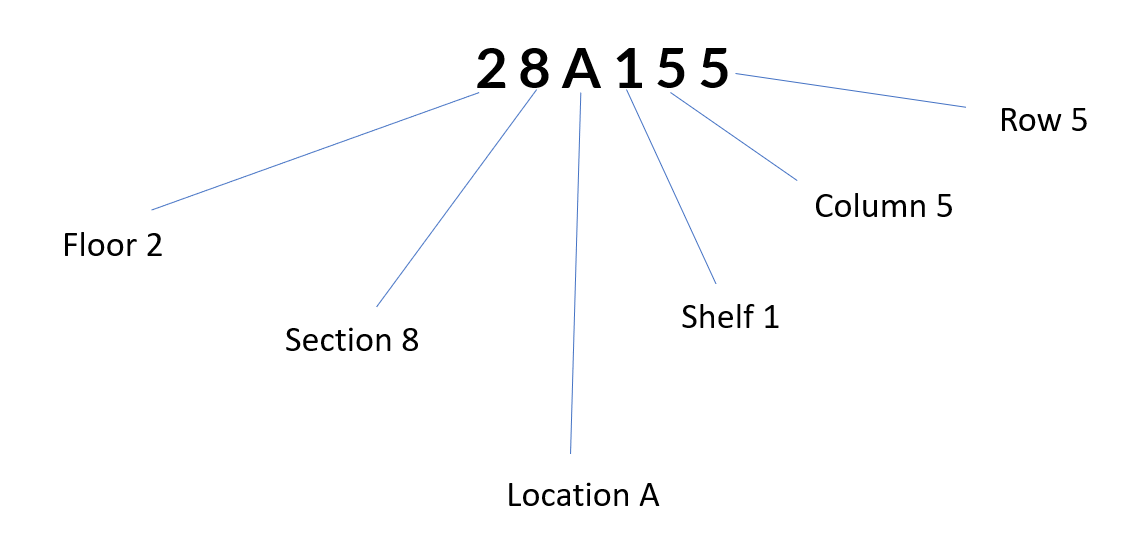
\includegraphics[scale=0.45]{figure/sample1.png}
        \caption{A slot in section 8, location A}
        \label{fig:sample1}
    \end{figure}

    \begin{figure}[!ht]
        \centering
        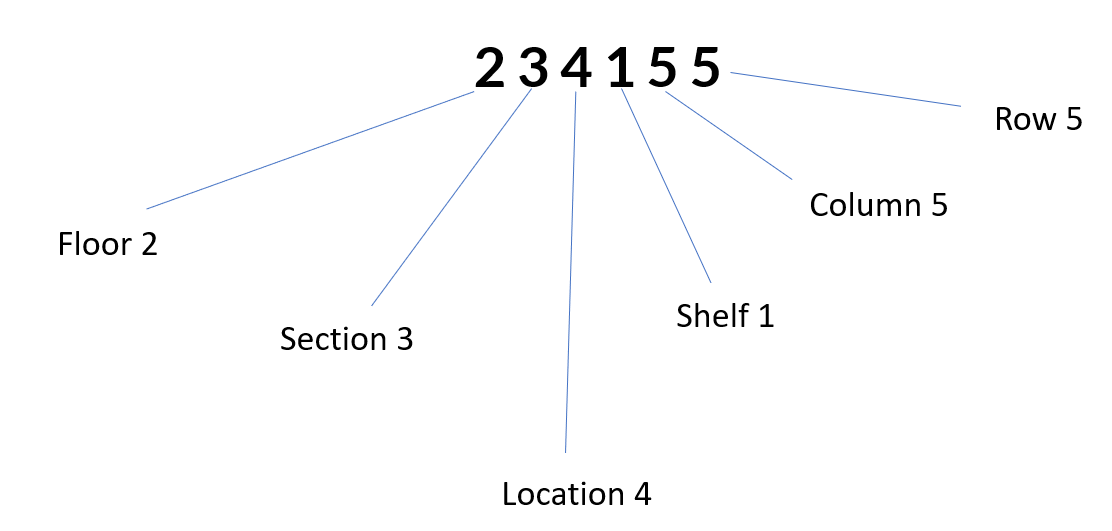
\includegraphics[scale=0.45]{figure/sample2.png}
        \caption{A slot in section 3, location 4}
        \label{fig:sample2}
    \end{figure}

The coordinate slot range from 11111 to 38D455 is established with limits and exception (as shown in table \ref{tab:coordinate}). These limits will provide a clear framework for locating and organizing items within the warehouse, which will help to improve efficiency and productivity.

    \begin{table}[H]
        \centering
        \caption{Coordinates}
        \begin{tabularx}{1\textwidth}{
            | >{\centering}a%\arraybackslash}y
            | >{\centering\arraybackslash}y
            | >{\centering\arraybackslash}y
            | >{\centering\arraybackslash}a|
            }
                \hline
            \bfseries  Type   
            &\bfseries Minimum  
            &\bfseries Maximum 
            & \bfseries Exception \\\hline
             Floor  & 1  & 3  &  \\\hline
             Section  & 1  & 8  &  \\\hline
             Location  & 1  & 7  & A,B,C,D (Section 8) \\\hline
             Shelf  & 1  & 4  &  \\\hline
             Column  & 1  & 5  &  \\\hline
             Row  & 1  & 5  &  \\\hline
        \end{tabularx}
        \label{tab:coordinate}
    \end{table}

\subsubsection{Layout}

\paragraph{Slot}\mbox{}

The following properties of both the slot and the item stored in the slot should be taken into consideration.

    Slot coordinate:
    \begin{equation}\label{eq:slot coordinate}
        X_s(i) = \text{ [Floor][Section][Location][Shelf][Column][Row]}
    \end{equation}

    Preferred item identification code to be stored:
    \begin{equation}\label{eq:pref IC}
        I_p(i) = \text{ [item code]}
    \end{equation}

    Denote if the slot is empty or not: 
    \begin{equation}\label{eq:empty}
        E_s(i) =  
        \begin{cases}
            1, & \text{ if there is item stored} \\
            0, & \text{ if there the slot is empty} \\
        \end{cases}
    \end{equation}
    
    Stored item identification code: 
    \begin{equation}\label{eq:stored item IC}
        I_s(i) =  
        \begin{cases}
            \text{ [item code]}, & \text{if  } E_s(i) = 1 \\
            0, & \text{if  } E_s(i) = 0 \\
        \end{cases}
    \end{equation}
        
    Stored carrier (carton box) identification code: 
    \begin{equation}\label{eq:storedcarrierIC}
        I_{sc}(i) =  
        \begin{cases}
            \text{ [carrier code]}, & \text{if  } E_s(i) = 1 \\
            0, & \text{if  } E_s(i) = 0 \\
        \end{cases}
    \end{equation}
    
    The timestamp when the item is stored:
    \begin{equation}\label{eq:stored timestamp}
        T_s(i) = \text{ [received timestamp]}
    \end{equation}
    
    Denote if the product is already reserved for order: 
    \begin{equation}\label{eq:reserved}
        R_d(i) =
        \begin{cases}
            1, & \text{ if stored item is reserved} \\
            0, & \text{ if stored item is not reserved} \\
        \end{cases}
    \end{equation}
        
    Order identification code: 
    \begin{equation}\label{eq:order IC}
        I_d(i) =  
        \begin{cases}
            \text{ [order code]}, & \text{if  } R_d(i) = 1 \\
            \text{ [null]}, & \text{if  } R_d(i) = 0 \\
        \end{cases}
    \end{equation}
    
    The estimate despatch timestamp, day, month, year: \quad 
    ${T_d(i), D_d(i), M_d(i), Y_d(i)}$

    Item shelf age at the date of calculation: 
    \begin{equation}\label{slot shelf age}
        T_a(i) = \text{ [now timestamp]} - T_s(i)
    \end{equation}

\paragraph{Column}\mbox{}
    
    Column coordinate:
    \begin{equation}\label{eq:column coordinate}
        X_c(i) = \text{ [Floor][Section][Location][Shelf][Column]}
    \end{equation}
    
    Preferred item identification code to be stored:
    \begin{equation}\label{eq:prefered column IC}
        I_c(i) = \text{ [item code]}
    \end{equation}

    Column storage capacity by slot: 
    \begin{equation}\label{eq:column capacity}
        C_c(i) = 5 - \sum_{j=1}^{5} E_s(f[X_c(i),j])
    \end{equation}

    Column age by the oldest product shelf age: 
    \begin{equation}\label{eq:column age}
        T_c(i) = max[T_a(f[X_c(i)])]
    \end{equation}

\paragraph{Shelf}\mbox{}

    Shelf coordinate:
    \begin{equation}\label{eq:shelf coordinate}
        X_f(i) = \text{ [Floor][Section][Location][Shelf]}
    \end{equation}
    
    Shelf storage capacity by slot: 
    \begin{equation}\label{eq:shelf capacity}
        C_f(i) = \sum_{j=1}^{5} C_c(f[X_f(i),j])
    \end{equation}

\paragraph{Location}\mbox{}

    Location coordinate:
    \begin{equation}\label{eq:location coordinate}
        X_n(i) = \text{ [Floor][Section][Location]}
    \end{equation}
    
    Location storage capacity by slot: 
    \begin{equation}\label{eq:location capacity}
        C_n(i) = \sum_{j=1}^{4} C_f(f[X_n(i),j])
    \end{equation}

\subsubsection{Parameters}

It is important to ensure that the warehouse does not operate at full capacity at all times, as this can lead to potential issues in the event of an emergency. Therefore, we recommend designating specific areas within the warehouse as emergency storage locations. In this case, we suggest assigning locations A, B, C, and D as emergency storage areas, along with the slots within those areas. By designating these specific locations as emergency storage, we can ensure that there is always enough space available to accommodate unexpected inventory or other urgent needs. This will help to ensure that the warehouse can operate safely and efficiently, even in the event of an emergency.

    Total slots: \quad
    ${ S_{t} = 18000 }$

    Available slots for allocate: \quad
    ${S_{a} = 16800}$

    Emergency slots: \quad
    ${ S_{e} = 1200 = \frac{1}{15} S_{t} }$

    Total number of product: \quad
    ${ W = 434 }$

\subsubsection{Product}

    Item code: \quad
    ${ I(i) }$
    
    Number of product per carrier: \quad
    ${ U(i) }$
    
    Price of each product: \quad
    ${ P_e(i) }$

    Price of each carrier:
    \begin{equation}\label{eq:price}
        P(i) = P_e(i) \times U(i)
    \end{equation}
    
    Cost of each product: \quad
    ${ A_e(i) }$
    
    Cost of each carrier:
    \begin{equation}\label{eq:cost}
        A(i) = A_e(i) \times U(i)
    \end{equation}
    
    Product profit per carrier:
    \begin{equation}\label{eq:profit}
        B(i) = P(i) - A(i)
    \end{equation}

\paragraph{Statistic}\mbox{}

    Total number of stored carrier of the product in the warehouse: 
    \begin{equation}\label{eq:Qs}
        Q_s(i) = \sum_{j=1}^{S_t}
        \begin{cases}
            E_s(j), & \text{if  } I(i) = I_s(j) \\
            0, & \text{if  } I(i) \neq I_s(j) \\
        \end{cases}
    \end{equation}

    Total number of reserved carrier of the product in the warehouse:
    \begin{equation}\label{eq:Qd}
        Q_d(i) = \sum_{j=1}^{S_t}
        \begin{cases}
            R_d(j), & \text{if  } I(i) = I_s(j) \\
            0, & \text{if  } I(i) \neq I_s(j) \\
        \end{cases}
    \end{equation}
    
    Total number of available carrier of the product in the warehouse: 
    \begin{equation}\label{eq:Qa}
        Q_a(i) = Q_s(i) - Q_d(i)
    \end{equation}

    Oldest available carrier coordinate:
    \begin{equation}\label{eq:Xo}
        X_o(i) = X(j), \quad \text{ if }
        \begin{cases}
            I(i) = I_s(j) \\
            R_d(j) = 0 \\
            T_a(j) = max[T_a(f[I(i)])] \\
        \end{cases}
    \end{equation}

    Newest stored carrier coordinate:
    \begin{equation}\label{eq:Xt}
        X_t(i) = X(j), \quad \text{ if }
        \begin{cases}
            I(i) = I_s(j) \\
            R_d(j) = 0 \\
            T_s(j) = min[T_s(f[I(i)])] \\
        \end{cases}
    \end{equation}

\paragraph{Record}\mbox{}

    Number of days each year: \quad
    ${ Z_{Y_d(j)} }$ (days) \quad <example: ${Z_{2022} = 365}$ days)>

    Total number of days since recorded: \quad
    \begin{equation}\label{eq:Zr}
        Z_r = \sum Z_{Y_d(j)} \text{ (days)}
    \end{equation}

    Number of orders product appear on each year: \quad
    ${ O_{Y_d(j)}(i) }$ (orders)

    Total number of orders involved since recorded:
    \begin{equation}\label{eq:Or}
        O_r(i) = \sum O_{Y_d(j)}(i) \text{ (orders)}
    \end{equation}

    Number of days product appear on order each year: \quad
    ${ D_{Y_d(j)}(i) }$ (days)

    Total number of days involved since recorded: \quad
    \begin{equation}\label{eq:Dr}
        D_r(i) = \sum D_{Y_d(j)}(i) \text{ (days)}
    \end{equation}

    The number of days involved will not exceed the number of orders involved:
    \begin{equation}\label{eq:leqdayorderannual}
        D_{Y_d(j)}(i) \leq O_{Y_d(j)}(i)
    \end{equation}
    \begin{equation}\label{eq:leqdayorderall}
        D_r(i) \leq O_r(i)
    \end{equation}

    Number of carrier despatched each year: \quad
    ${ Q_{Y_d(i)}(i) }$ (carriers)

    Total number of carrier despatched recorded: \quad
    \begin{equation}\label{eq:Qr}
        Q_r(i) = \sum Q_{Y_d(j)}(i) \text{ (carriers)}
    \end{equation}

    It is important to note that:
    \begin{equation}\label{eq:leqQYd}
        \sum_{i=1}^{W} Q_{Y_d(j)}(i) \leq S_t \times Z_{Y_d(j)}
    \end{equation}
    \begin{equation}\label{eq:leqQr}
        \sum_{i=1}^{W}Q_{r(j)}(i) \leq S_t \times Z_{r}
    \end{equation}

    The frequency, or ratio of appearance of the product:
    \begin{equation}\label{eq:FYd}
        F_{Y_d(j)}(i) = \frac{D_{Y_d(j)}(i)}{Z_{Y_d(j)}}
    \end{equation}
    \begin{equation}\label{eq:Fr}
        F_r(i) = \frac{D_r(i)}{Z_r}
    \end{equation}

    The average flow of product:
    \begin{equation}\label{eq:GYd}
        G_{Y_d(j)}(i) = \frac{Q_{Y_d(j)}(i)}{O_{Y_d(j)}(i)} \text{ (carrier per order)}
    \end{equation}
    \begin{equation}\label{eq:Gr}
        G_r(i) = \frac{Q_r(i)}{O_r(i)} \text{ (carrier per order)}
    \end{equation}
    \begin{equation}\label{eq:gYd}
        g_{Y_d(j)}(i) = \frac{Q_{Y_d(j)}(i)}{D_{Y_d(j)}(i)} \text{ (carrier per day)}
    \end{equation}
    \begin{equation}\label{eq:gr}
        g_r(i) = \frac{Q_r(i)}{D_r(i)} \text{ (carrier per day)}
    \end{equation}
    
    Combined with equation \eqref{eq:leqdayorderannual} and \eqref{eq:leqdayorderall}:
    \begin{equation}\label{eq:geqgYd}
        g_{Y_d(j)}(i) \geq G_{Y_d(j)}(i)
    \end{equation}
    \begin{equation}\label{eq:geqgr}
        g_{r(j)}(i) \geq G_{r(j)}(i)
    \end{equation}

    The average slot demand of product:
    \begin{equation}\label{eq:HYd}
        H_{Y_d(j)}(i) = \frac{Q_{Y_d(j)}(i)}{Z_{Y_d(j)}}
        \text{ (slot per day)}
    \end{equation}
    \begin{equation}\label{eq:Hr}
        H_r(i) = \frac{Q_r(i)}{Z_r}
        \text{ (slot per day)}
    \end{equation}

\subsection{Control objective}

\subsubsection{Space allocation}

    Total average slot demand of all products:
    \begin{equation}\label{eq:VYd}
        V_{Y_d(j)} = \sum_{k=1}^{W} H_{Y_d(j)}(k) 
        = \sum_{k=1}^{W} \frac{Q_{Y_d(j)}(i)}{Z_{Y_d(j)}}
        \leq S_t
    \end{equation}
    
    \begin{equation}\label{eq:Vr}
        V_r = \sum_{k=1}^{W} H_r(k) 
        = \sum_{k=1}^{W} \frac{Q_{r}(i)}{Z_{r}}
        \leq S_t
    \end{equation}

    Total stored slot in the warehouse at the current date:
    \begin{equation}\label{eq:Vs}
        V_s = \sum_{j=1}^{S_a} E_s(j) \leq S_a
    \end{equation}

    Total empty slot in the warehouse at the current date:
    \begin{equation}\label{eq:Ve}
        V_e = S_a - V_s
    \end{equation}

    Total emergency slot in use at the current date:
    \begin{equation}\label{eq:Vemc}
        V_{emc} = \sum E_s(f[X_{emc}]) \leq S_e
    \end{equation}

    Total empty column in the warehouse at the current date:
    \begin{equation}\label{eq:Ke}
        K_e = \sum_{i=1}^{3360}
        \begin{cases}
            1, & \text{if } C_c(i) = 5 \\
            0, & \text{if } C_c(i) < 5 \\
        \end{cases}
        \quad \text{ also } K_e \leq \frac{V_e}{5}
    \end{equation}

\paragraph{First cycle}\mbox{}

    In case ${ V_s = 0 }$
            
    All time value of each product:
    \begin{equation}\label{eq:Nri}
        N_r(i) = Q_r(i) \times B(i)
    \end{equation}

    All time value of all products:
    \begin{equation}\label{eq:Nr}
        N_r = \sum_{i=1}^{W} N_r(i) 
    \end{equation}

    Percentage of all time value for each product:
    \begin{equation}\label{eq:Lri}
        L_r(i) = \frac{N_r(i)}{N_r}
    \end{equation}

    In accord to the annual percentage ${ L_r(i) }$ and frequency ${ F_r(i) }$ of each product, which is sorted from high to low. Applying ABC analysis method, the number of columns allocate to each product can be calculated.
    \begin{equation}\label{eq:K}
        K(i) = 
        \begin{cases}
            \frac{max[g_r(i),H_r(i)]}{5}, & 
            \text{case A} \\
            \frac{max[G_r(i),H_r(i)]}{5}, & 
            \text{case B} \\
            \frac{min[G_r(i),H_r(i)]}{5}, & 
            \text{case C} \\
        \end{cases}
    \end{equation}

    As long as the following condition is sastified:
    \begin{equation}\label{eq:conditionK}
        \sum_{i=1}^{W} K(i) \leq \frac{S_a}{5}
    \end{equation}

    Further elaborate with equation \eqref{eq:Gr} and \eqref{eq:Vr} in case C of equation \eqref{eq:K}:
    \begin{equation}\label{eq:elaborate first cycle}
        \sum_{i=1}^{W} min[G_r(i),H_r(i)] \leq 
        \sum_{k=1}^{W} H_{Y_r}(i)
        \leq S_t
    \end{equation}

    Also statistic report in 2019 (appendix A) show that:
    \begin{equation}\label{eq:report 2019}
        \sum_{i=1}^{W} U(i) \times Q_{2019}(i) = 75982216, 
        \text{ with } U_{avg} \approx 458
    \end{equation}

    Hence average slot demand of all products in 2019:
    \begin{equation}\label{eq:sample 2019}
        V_{2019} = \sum_{i=1}^{W} \frac{Q_{2019}(i)}{Z_{2019}} \approx 165900 
        \approx \frac{1}{39,6} \times S_t
    \end{equation}

\paragraph{Annual cycle}\mbox{}

    Previous year:
    \begin{equation}\label{eq:Yp}
        Y_p = 2022 \text{ (sample)}
    \end{equation}

    Annual value of each product:
    \begin{equation}\label{eq:NYpi}
        N_{Y_p}(i) = Q_{Y_p}(i) \times B(i)
    \end{equation}

    Annual value of previous year:
    \begin{equation}\label{eq:NYp}
        N_{Y_p} = \sum_{i=1}^{W} N_{Y_p }(i) 
    \end{equation}

    Percentage of annual value for each product:
    \begin{equation}\label{eq:LYpi}
        L_{Y_p}(i) = \frac{N_{Y_p }(i)}{ N_{Y_p }}
    \end{equation}

   In accord to the annual percentage ${ L_{Y_p}(i) }$ and frequency ${ F_{Y_p}(i) }$ of each product, which is sorted from high to low. Applying ABC analysis method, the number of columns allocate to each product can be calculated.
    \begin{equation}\label{eq:Ka}
        K_a(i) = 
        \begin{cases}
            K_e \times \frac{max[g_{Y_p}(i),H_{Y_p}(i)]}{S_a}, & 
            \text{case A} \\
            K_e \times \frac{max[G_{Y_p}(i),H_{Y_p}(i)]}{S_a}, & 
            \text{case B} \\
            K_e \times \frac{min[G_{Y_p}(i),H_{Y_p}(i)]}{S_a}, & 
            \text{case C} \\
        \end{cases}
    \end{equation}
    
    As long as the following condition is sastified:
    \begin{equation}\label{eq:ConditionKa}
        \sum_{i=1}^{W} K_a(i) \leq K_e
    \end{equation}

It is worth noting that the annual cycle can be adjusted to a quarterly or monthly cycle to allow for more flexible space allocation. By adjusting the cycle to a shorter timeframe, it becomes easier to adjust warehouse operations based on changes in inventory needs and other factors. This can help to optimize space allocation and improve overall warehouse efficiency.

\subsubsection{Receiving and put-away}

Although TPP plastic products have a lifespan of about 50 years, it is still important to have a storage strategy in place to prevent products from sitting on the shelf for too long. Therefore, a FIFO (first in, first out) strategy has been chosen to ensure that older products are used or sold before newer ones.

Based on the FIFO strategy, the following variables are to be considered when the system receives a new carrier: product identification code ${ I }$ and the corresponding product newest stored coordinate ${ X_t }$.

    Find youngest column with suitable capacity (there is empty slot within):
    \begin{equation}\label{eq:rap find X}
        X = 
        \begin{cases}
            f[X_c(f[X_t])], & \text{if } C_c(f[X_t]) > 0 \\
            f[X_c(j)], & \text{if }
            \begin{cases}
                C_c(f[X_t]) = 0 \\
                T_c(j) = min[T_c(f[I])] \\
                C_c(j) > 0 \\
            \end{cases}
        \end{cases}
    \end{equation}

In case there are multiple empty columns as well as full columns that have been designated for a specific product, it is recommend to select the empty column that is closest to the full ones:
    \begin{equation}\label{eq:empty find X}
        X = f[X_c(j)], \quad
            \begin{cases}
                C_c(f[I]) = 0 \\
                C_c(f'[I]) = 5 \\
                |j-f[I]| \text{ is minimum}
            \end{cases}
    \end{equation}

\subsubsection{Order fulfillment}

There are two scenarios: either the total available product carrier ${ Q_a(i) }$ is \linebreak sufficient to fulfill the order, or it is insufficient.

\paragraph{Sufficient}\mbox{}

When considering the age column, columns ${ X_c(i) }$ are selected from the oldest to the youngest <${ T_c(i) }$>. In each column, carriers ${ X(i) }$ are selected using the same principle <${ T_a(i) }$>.

    Hence, there is no emergency request send to the factory:
    \begin{equation}\label{eq:no emc}
        \text{\emph{EMC(i)}} =  0
    \end{equation}

\paragraph{Insufficient}\mbox{}

Place a replenishment request for the emergency locations. Carriers in here should be placed order by order, with priority given to the first order to be picked.
    \begin{equation}\label{eq:emc}
        \text{\emph{EMC(i)}} =  
        \text{\emph{order numbers (i)}} - Q_a(i)
    \end{equation}

    Provided that the following condition is met:
    \begin{equation}\label{eq:sum emc}
        \sum EMC_{D_d} \leq \text{\emph{ factory capacity}}
    \end{equation}

\subsubsection{Daily replenishment}

To calculate the daily replenishment for the warehouse, both the factory capacity and emergency requests need to be taken into consideration.
    \begin{equation}\label{eq:drq}
        \text{\emph{daily replenishment quota}} = 
        \text{\emph{factory capacity}} - \sum EMC{D_d} 
    \end{equation}

Based on the product frequency from the previous year ${ F_{Y_d} }$, products should be picked in order of higher frequency, while ensuring that the total replenishment does not exceed the quota.
    \begin{equation}\label{eq:quota}
        \sum C_c(i) = \sum (5 \times K_a(i)) + \sum C_{c,prev}(i)
        \leq \text{\emph{ daily replenishment quota}}
    \end{equation}

\subsection{Control algorithm}

\subsubsection{Space allocation}\label{ca:space allocation}

In the control loop shown in \autoref{fig:Space allocation control loop}, the input is the serial number of the product, and the output is the number of columns assigned to the product. The controller uses the annual percentage and frequency of each product, applying the ABC analysis method with equation \eqref{eq:conditionK} and \eqref{eq:ConditionKa} to generate a control signal that determines the output. The output is calculated using equation \eqref{eq:K} and \eqref{eq:Ka}.

    Control loop for space allocation cycle:
    \begin{figure}[!ht]
        \centering
        \begin{tikzpicture}[auto, node distance=2cm,>=latex']
            \node [input, name=input] 
            {};
            \node [block, right of=input, node distance=3cm] (controller) 
            {$f[L(i),F(i)]$};
            \node [block, right of=controller, node distance=5cm] (system) 
            {$f[g(i),G(i),H(i)]$};
            \node [output, right of=system, node distance=4cm] (output) 
            {};
            \draw [draw,->] (input) -- node 
            {$i$} (controller);
            \draw [->] (controller) -- node[name=u, above] 
            {$u$} (system);
            \draw [->] (system) -- node [name=y, above] 
            {$K(i)$}(output);
        \end{tikzpicture}
        \caption{Space allocation control loop block diagram}
        \label{fig:Space allocation control loop}
    \end{figure}

\subsubsection{Receiving and put-away}\label{ca:receiving and put-away}

Based on \autoref{fig:Receiving and put-away flowchart diagram}, the algorithm takes information about the new carrier as input and outputs the coordinate where the system will place it. The algorithm finds the most suitable slot that satisfies the FIFO strategy from the column that stores or is assigned to the same item.

A control algorithm for the receiving and put-away process was designed using equations \eqref{eq:rap find X} and \eqref{eq:empty find X}:
    \begin{figure}[!ht]
        \centering
        \begin{tikzpicture}[node distance=2cm]

        \node (start) [startstop] 
        {Receiving};
        \node (input) [io, below of = start] 
        {New Carrier};
        \node (proc1) [process, below of = input] 
        {find $I$ and ${X_t}$};
        \node (dec2) [decision, below of = proc1, yshift = -1cm] 
        {${C_c(f[X_t]) > 0}$};
    
        \node (proc2y) [process, below of = dec2, yshift = -2cm] 
        {find ${X_c(f[X_t])}$};
        \node (output) [io, below of=proc2y] 
        {${X=f[X_c]}$};
        \node (stop) [startstop, below of=output] 
        {Put-away};
                
        \node (proc2n) [process, right of = dec2, xshift = 4cm] 
        {filter ${k = f[I]}$ \\ ${5 \geq C_c(k) > 0}$};
        \node (proc3) [process, below of = proc2n, yshift = -2cm] 
        {find ${T_c(j) = min[T_c(k)]}$ or \linebreak ${|j-f[I]}$ is minimum};
        \node (proc4) [process, below of = proc3, yshift = 0cm] 
        {find ${X_c(j)}$};
        
        \draw [arrow] (start) -- (input);
        \draw [arrow] (input) -- (proc1);
        \draw [arrow] (proc1) -- (dec2);
        \draw [arrow] (dec2) -- node[anchor=east] {yes} (proc2y);
        \draw [arrow] (dec2) -- node[anchor=south] {no} (proc2n);
        \draw [arrow] (proc2y) -- (output);
        \draw [arrow] (output) -- (stop);
        
        \draw [arrow] (proc2n) -- (proc3);
        \draw [arrow] (proc3) -- (proc4);
        \draw [arrow] (proc4) -- (output);
        
        \end{tikzpicture}
        \caption{Receiving and put-away flowchart diagram}
        \label{fig:Receiving and put-away flowchart diagram}
    \end{figure}

\subsubsection{Order fulfillment}\label{ca:order fulfillment}

Based on the flowchart diagram for order fulfillment shown in \autoref{fig:Order fulfillment flowchart diagram}, the algorithm takes the product identification code from a new order as its input and outputs the locations where the system will pick the products. The algorithm finds the most suitable slot that satisfies the FIFO strategy and requests more products from the factory in cases where there are insufficient numbers.

A control algorithm for order fulfillment process is designed based on equations \eqref{eq:no emc}, \eqref{eq:emc}, and \eqref{eq:sum emc}:
    \begin{figure}[!ht]
        \centering
        \begin{tikzpicture}[node distance=2cm]

        \node (start) [startstop] 
        {Fulfill};
        \node (input) [io, below of = start] 
        {New Order};
        \node (proc1) [process, below of = input] 
        {find $I(i)$ and $n(i)$ of each product};
        \node (dec2) [decision, below of = proc1, yshift = -2cm] 
        {${Q_a(f[I(i)]) \geq n(i)}$};
    
        \node (proc2y) [io, below of = dec2, yshift = -2cm] 
        {${EMC(i) = 0}$};
        \node (output) [io, below of=proc2y] 
        {${X=X_o(f[I(i)])}$};
        \node (stop) [startstop, below of=output] 
        {Picking};
                
        \node (proc2n) [io, right of=dec2, xshift=4cm, text width=4cm, align=center]
        {${EMC(i) = }$ \linebreak ${n(i) - Q_a(f[I(i)])}$};
        \node (proc3) [process, below of = proc2n, yshift = -2cm] 
        {sent \\ emergency request};
        \node (proc4) [process, below of = proc3, yshift = 0cm] 
        {delay };
        \node (dec3) [decision, below of = proc4, yshift = -2cm]
        {sufficient};
        \node (emc) [io, left of = dec3, xshift = -4cm]
        {emergency location};
        
        \draw [arrow] (start) -- (input);
        \draw [arrow] (input) -- (proc1);
        \draw [arrow] (proc1) -- (dec2);
        \draw [arrow] (dec2) -- node[anchor=east] 
        {yes} (proc2y);
        \draw [arrow] (dec2) -- node[anchor=north] 
        {no} (proc2n);
        \draw [arrow] (proc2y) -- (output);
        \draw [arrow] (output) -- (stop);

        \draw [arrow] (proc2n) -- (proc3);
        \draw [arrow] (proc3) -- (proc4);
        \draw [arrow] (proc4) -- (dec3);

        \draw [arrow] (dec3) -- node[anchor=north] 
        {yes} (emc);
        \draw [arrow] (dec3) -- ++(3cm,0) |- node[anchor=west] 
        {no} (proc4);
        \draw [arrow] (emc) -- (stop);
        
        \end{tikzpicture}
        \caption{Order fulfillment flowchart diagram}
        \label{fig:Order fulfillment flowchart diagram}
    \end{figure}

\subsubsection{Daily replenishment}\label{ca:replenishment}

In the control loop depicted in \autoref{fig:Replenishment control loop}, the input, or set point, is the total available slots for allocation. The feedback signal is the total number of stored slots (excluding emergency slots), which is calculated using equation \eqref{eq:Vs}. The output is the daily replenishment request sent to the factory. The disturbance is the emergency request. The error signal is the total number of empty slots (excluding emergency slots), calculated using equation \eqref{eq:Ve}. The actuating signal is the storage capacity of columns, calculated using equation \eqref{eq:column capacity}. The controller uses the product frequency to prioritize which product to replenish first.

    Replenishment control loop:
    \begin{figure}[!ht]
        \centering
        \begin{tikzpicture}[auto, node distance=2cm,>=latex']
            \node [input, name=input] 
            {};
            \node [sum, right of=input, node distance=1cm] (sum) 
            {};
            \node [block, right of=sum, node distance=3cm] (controller) 
            {$f[F(i)]$};
            \node [block, right of=controller, 
            pin={[pinstyle]above:$ \sum EMC_{D_d} $},
                node distance=6cm] (system) 
            {\emph{factory}};
            \draw [->] (controller) -- node[name=u, above] 
            {$C_c(f[F(i)])$} (system);
            \node [output, right of=system, node distance=5cm] (output) 
            {};
            \node [block, below of=u] (measurements) 
            {$f[E_s(j)]$};
            \draw [draw,->] (input) -- node 
            {$S_a$} (sum);
            \draw [->] (sum) -- node 
            {$V_e$} (controller);
            \draw [->] (system) -- node [name=y, above] 
            {\emph{replenishment}}(output);
            \draw [->] (y) |- (measurements);
            \draw [->] (measurements) -| node[pos=0.99] 
            {$-$} 
                node [near end] 
            {$V_s$} (sum);
        \end{tikzpicture}
        \caption{Replenishment control loop block diagram}
        \label{fig:Replenishment control loop}
    \end{figure}

\newpage